\chapter{Операторы, наблюдаемые величины и матрицы Паули}

Хорошая система обозначений — не украшение. В дисциплине, построенной на абстрактных векторах и комплексных числах, обозначения, позволяющие нам оперировать символами, не переводя их каждый раз в слова, составляют часть самого аппарата. Обозначения Дирака бра--кет ценны именно по этой причине: они сохраняют на виду геометрию пространства состояний, позволяя при этом вычислять с компонентами и матрицами.

Наша ближайшая задача — математическая. Мы введём линейные операторы, выясним, как они действуют не только на кеты, но и на бра, и выделим особый класс, называемый эрмитовыми операторами. Лишь затем мы присоединим физические слова — \emph{наблюдаемая величина}, \emph{результат измерения} и \emph{вероятность}. В награду мы увидим, что три спиновые наблюдаемые величины возникают как матрицы Паули, а не выдаются нам как объекты для заучивания.

\section{Ортонормированные базисы и компоненты}

Состояния образуют комплексное линейное векторное пространство. Его кет-векторы можно складывать и умножать на комплексные числа. Каждому кету \(\ket{A}\) сопоставлен бра \(\bra{A}\), получаемый операцией сопряжённого двойствования. Базис не единственен, но после его выбора каждый вектор можно описать его компонентами в этом базисе.

Пусть
\[
\bigl\{\ket{1},\ket{2},\ldots,\ket{N}\bigr\}
\]
— ортонормированный базис. Ортогональность и нормировка выражаются соотношением
\begin{equation}
\braket{j}{i}=\delta_{ji}.
\label{eq:orthonormal-basis}
\end{equation}
Здесь \(\delta_{ji}\) равно единице при \(j=i\) и нулю в противном случае. Размерность \(N\) — это максимальное число взаимно ортогональных направлений в пространстве; полный ортонормированный базис содержит ровно столько векторов.

Разложим произвольный кет в виде
\begin{equation}
\ket{A}=\sum_i \alpha_i\ket{i}.
\label{eq:ket-expansion}
\end{equation}
Коэффициенты здесь вовсе не загадочны. Домножим слева на \(\bra{j}\):
\begin{align}
\braket{j}{A}
 &=\sum_i\alpha_i\braket{j}{i} \\
 &=\sum_i\alpha_i\delta_{ji}
 =\alpha_j.
\end{align}
Следовательно,
\begin{equation}
\alpha_i=\braket{i}{A}.
\label{eq:components-inner-products}
\end{equation}
Компонента с номером \(i\) — это проекция \(\ket{A}\) на \(i\)-е направление базиса.

Подстановка уравнения~\eqref{eq:components-inner-products} обратно в уравнение~\eqref{eq:ket-expansion} даёт особенно полезную форму
\begin{equation}
\ket{A}=\sum_i\ket{i}\braket{i}{A}.
\label{eq:ket-completeness-action}
\end{equation}
Сумма ничего не сделала с вектором; она лишь разложила его по базисным направлениям, а затем снова собрала. Мы будем многократно пользоваться этой операцией. Обычно это описывают как \emph{вставку полного набора состояний}, поскольку
\begin{equation}
\sum_i\ket{i}\bra{i}=\mathbf 1.
\label{eq:resolution-identity}
\end{equation}

Соответствующее разложение для бра имеет вид
\begin{equation}
\bra{A}=\sum_i\braket{A}{i}\bra{i}
       =\sum_i\alpha_i^*\bra{i}.
\label{eq:bra-expansion}
\end{equation}
Комплексное сопряжение у \(\alpha_i\) существенно. При переходе от кета к бра каждый числовой коэффициент комплексно сопрягается.

\begin{figure}[htbp]
\centering
\includegraphics[width=0.82\textwidth]{lecture_03_figure_04.png}
\caption{Два определяющих правила линейного оператора, записанные после обзора базиса.}
\lectureframe{00:12:44}
\end{figure}

\section{Линейные операторы как машины}

Линейный оператор \(M\) — это правило, сопоставляющее каждому входному кету единственный выходной кет. Полезный образ, предложенный Джоном Уилером, — это машина с входным и выходным портами: вставьте \(\ket{A}\), поверните колесо и получите \(M\ket{A}\). Выход однозначно определяется входом. Обратное соответствие не обязано быть однозначным; два входа могут давать один и тот же выход, и обратной машины может не существовать.

Слово \emph{линейный} означает два правила. Для комплексного числа \(z\),
\begin{align}
M\bigl(z\ket{A}\bigr)&=z\,M\ket{A}, \label{eq:operator-homogeneous}\\
M\bigl(\ket{A}+\ket{B}\bigr)&=M\ket{A}+M\ket{B}.
\label{eq:operator-additive}
\end{align}
Скаляр проходит через машину без изменения, а сумму можно обрабатывать по одному слагаемому. Эти правила также влекут линейность любой конечной комплексной линейной комбинации.

То же самое относится и к обычным трёхмерным векторам. Квантовая механика не изобретает линейные отображения. Она делает их незаменимыми, потому что пространство состояний абстрактно и комплексно, а измеримые величины будут представлены выделенным семейством таких отображений.

\section{От оператора к его матрице}

Предположим, что машина переводит \(\ket{A}\) в \(\ket{B}\):
\begin{equation}
M\ket{A}=\ket{B}.
\label{eq:operator-action}
\end{equation}
Выберем один и тот же ортонормированный базис для входа и выхода и запишем
\[
\ket{A}=\sum_j\alpha_j\ket{j},
\qquad
\ket{B}=\sum_i\beta_i\ket{i}.
\]
Чтобы найти \(i\)-ю компоненту выхода, спроецируем уравнение~\eqref{eq:operator-action} с помощью \(\bra{i}\):
\begin{equation}
\bra{i}M\ket{A}=\braket{i}{B}=\beta_i.
\end{equation}
Теперь подставим разложение \(\ket{A}\):
\begin{align}
\bra{i}M\ket{A}
 &=\sum_j\bra{i}M\ket{j}\braket{j}{A}\\
 &=\sum_j\bra{i}M\ket{j}\alpha_j
 =\beta_i.
\end{align}
Числа
\begin{equation}
m_{ij}\equiv\bra{i}M\ket{j}
\label{eq:matrix-elements}
\end{equation}
являются \emph{матричными элементами} оператора \(M\) в выбранном базисе. Следовательно,
\begin{equation}
\boxed{\sum_jm_{ij}\alpha_j=\beta_i.}
\label{eq:component-action}
\end{equation}

\begin{figure}[htbp]
\centering
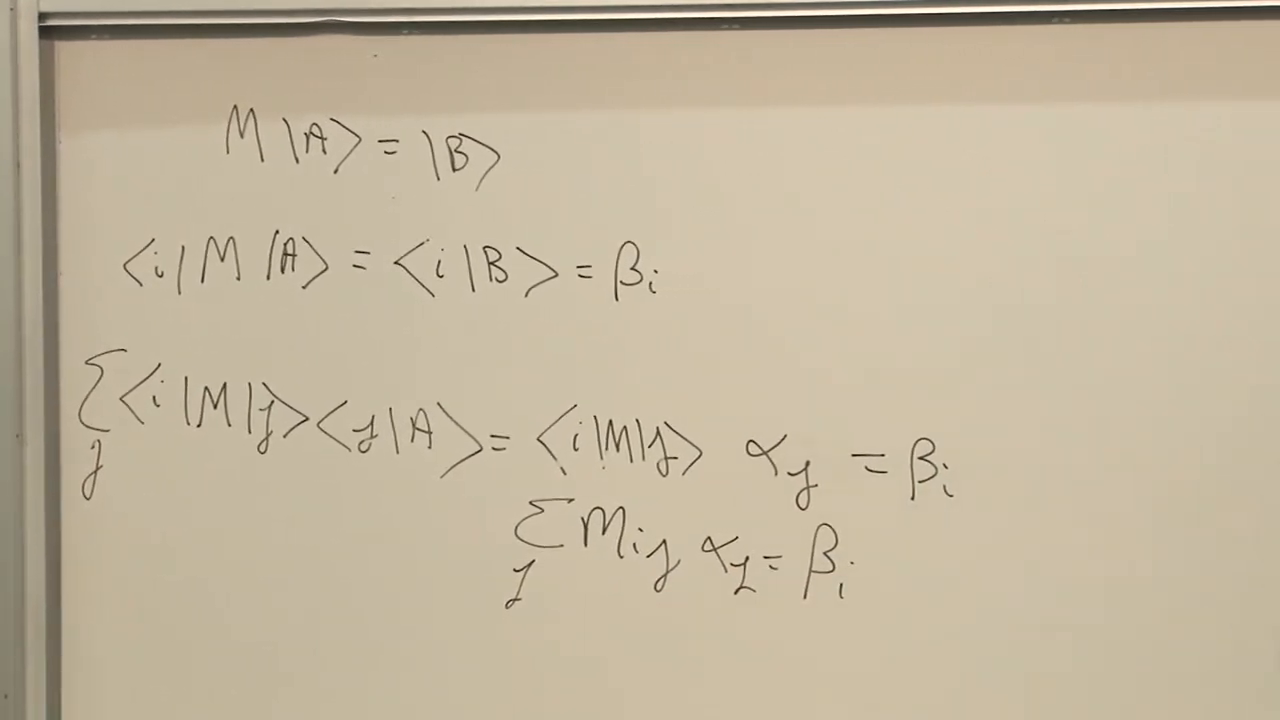
\includegraphics[width=0.84\textwidth]{lecture_03_figure_02.png}
\caption{Абстрактное уравнение \(M\ket{A}=\ket{B}\), спроецированное и разложенное в покомпонентное правило \(\sum_jm_{ij}\alpha_j=\beta_i\).}
\lectureframe{00:18:30}
\end{figure}

Если пространство имеет размерность \(N\), то \(N^2\) чисел \(m_{ij}\) образуют квадратную матрицу \(N\times N\). Уравнение~\eqref{eq:component-action} имеет в точности вид
\begin{equation}
\begin{pmatrix}
m_{11}&m_{12}&\cdots&m_{1N}\\
m_{21}&m_{22}&\cdots&m_{2N}\\
\vdots&\vdots&\ddots&\vdots\\
m_{N1}&m_{N2}&\cdots&m_{NN}
\end{pmatrix}
\begin{pmatrix}
\alpha_1\\
\alpha_2\\
\vdots\\
\alpha_N
\end{pmatrix}
=
\begin{pmatrix}
\beta_1\\
\beta_2\\
\vdots\\
\beta_N
\end{pmatrix}.
\label{eq:matrix-vector-action}
\end{equation}
Чтобы получить \(\beta_1\), умножьте первую строку на входной столбец и просуммируйте; затем повторите это со второй строкой для \(\beta_2\), и так далее. Матрица — конкретное воплощение машины Уилера.

\begin{figure}[htbp]
\centering
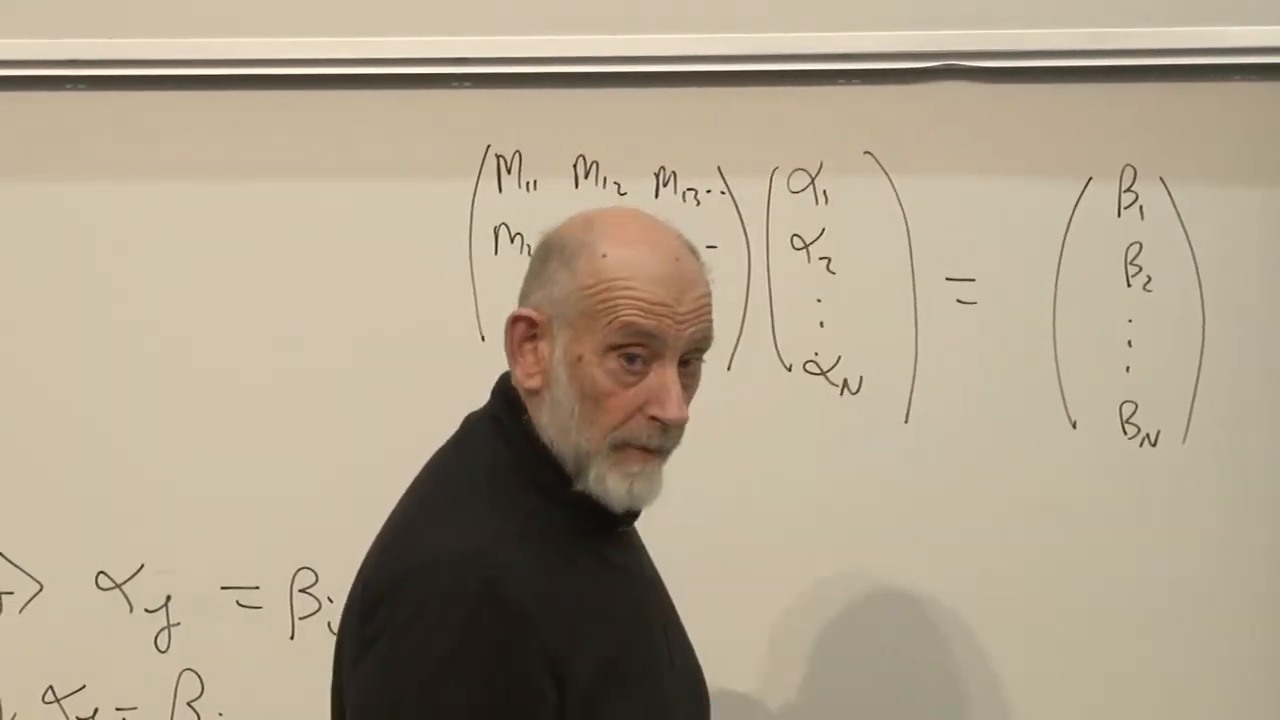
\includegraphics[width=0.84\textwidth]{lecture_03_figure_03.png}
\caption{То же действие оператора, представленное как умножение квадратной матрицы на столбец входных коэффициентов.}
\lectureframe{00:20:01}
\end{figure}

Мы приобрели алгоритм и потеряли часть наглядной геометрии. Абстрактное утверждение \(M\ket{A}=\ket{B}\) не зависит от координат. Конкретные величины \(m_{ij}\), \(\alpha_j\) и \(\beta_i\) зависят от выбранного базиса. Другой ортонормированный базис изменит все три набора, оставив лежащее в основе отображение и его физические предсказания неизменными.

\begin{classroomqa}
\audiencequestion{Может ли выбор базиса определять, можно ли решить задачу?}
\lecturerresponse{Он может определять, насколько легко увидеть решение. Удачно выбранный базис может сделать оператор диагональным, а вычисление почти непосредственным; неудачный базис может скрыть структуру за неприятной алгеброй. Изменить результат эксперимента он не может. Если два базиса приводят к разным физическим ответам, вычисление неверно.}
\end{classroomqa}

\section{Бра, кеты и антилинейность}

\begin{classroomqa}
\audiencequestion{Может ли линейный оператор превращать кет в бра или бра в кет?}
\lecturerresponse{Не обычный линейный оператор того типа, который мы только что определили. Он отображает кеты в кеты, причём комплексные скаляры проходят через него без изменения. Операция, которая меняет кеты и бра местами, также комплексно сопрягает их коэффициенты, так что она относится к другому классу.}
\end{classroomqa}

Умножение на фиксированное комплексное число — простой линейный оператор. Комплексное сопряжение таковым не является. Если \(K\) обозначает сопряжение, то
\[
K\bigl(z\ket{A}\bigr)=z^*K\ket{A},
\]
а не \(zK\ket{A}\). Такое отображение называется \emph{антилинейным}. Это название не означает противоположность линейному; оно лишь фиксирует сопряжение скаляров. Его более глубокая связь с античастицами выходит за рамки настоящего обсуждения.

Тем не менее действие линейных операторов можно определить и на бра. По соглашению оператор записывают справа:
\begin{equation}
\bra{A}M.
\end{equation}
Определение выбирают так, чтобы у матричного элемента не возникало неоднозначности со скобками:
\begin{equation}
\bra{A}\bigl(M\ket{B}\bigr)
=
\bigl(\bra{A}M\bigr)\ket{B}
\equiv
\bra{A}M\ket{B}.
\label{eq:bracket-independence}
\end{equation}

Чтобы понять, почему это возможно, разложим оба вектора:
\begin{align}
\bra{A}M\ket{B}
 &=\left(\sum_i\alpha_i^*\bra{i}\right)
   M
   \left(\sum_j\beta_j\ket{j}\right)\\
 &=\sum_{ij}\alpha_i^*m_{ij}\beta_j.
\label{eq:matrix-element-double-sum}
\end{align}
Это обычная двойная сумма. Можно сначала просуммировать по \(j\) и рассматривать \(M\) как действующий на кет, а можно сначала просуммировать по \(i\) и рассматривать оператор как действующий на бра. Результат один и тот же. Нотация устроена именно так, чтобы можно было убрать лишние скобки.

\section{Операция даггера}

Есть и второй, отличный от первого, вопрос, связанный с бра. Пусть
\[
M\ket{A}=\ket{B}.
\]
Какой оператор переводит соответствующий бра \(\bra{A}\) в \(\bra{B}\)? Вообще говоря, это не сам \(M\). Если бы \(M\) был умножением на комплексное число \(z\), то уравнение для кета имело бы вид \(\ket{B}=z\ket{A}\), тогда как уравнение для бра имело бы вид \(\bra{B}=z^*\bra{A}\).

Искомый оператор обозначают \(M^\dagger\) — оператор, \emph{эрмитово сопряжённый} к \(M\), — и определяют соотношением
\begin{equation}
M\ket{A}=\ket{B}
\quad\Longleftrightarrow\quad
\bra{A}M^\dagger=\bra{B}.
\label{eq:dagger-definition}
\end{equation}
Даггер — операторный аналог комплексного сопряжения.

Его матричное правило следует непосредственно. Пусть
\[
M\ket{i}=\ket{i'}.
\]
Тогда
\[
m_{ji}=\bra{j}M\ket{i}=\braket{j}{i'}.
\]
Соответствующее соотношение для бра имеет вид \(\bra{i}M^\dagger=\bra{i'}\), поэтому
\[
(m^\dagger)_{ij}
=\bra{i}M^\dagger\ket{j}
=\braket{i'}{j}.
\]
При перестановке местами векторов в скалярном произведении результат комплексно сопрягается:
\[
\braket{i'}{j}=\braket{j}{i'}^*.
\]
Следовательно,
\begin{equation}
\boxed{(m^\dagger)_{ij}=m_{ji}^*.}
\label{eq:dagger-matrix-elements}
\end{equation}

\begin{figure}[htbp]
\centering
\includegraphics[width=0.84\textwidth]{lecture_03_figure_05.png}
\caption{Итоговое записанное на доске соотношение для эрмитова сопряжения: поменять индексы местами и взять комплексное сопряжение.}
\lectureframe{00:42:23}
\end{figure}

На языке матриц нужно транспонировать, а затем взять комплексное сопряжение:
\begin{equation}
\begin{pmatrix}
a&b\\
c&d
\end{pmatrix}^{\!\dagger}
=
\begin{pmatrix}
a^*&c^*\\
b^*&d^*
\end{pmatrix}.
\label{eq:dagger-two-by-two}
\end{equation}
Транспонирование отражает элементы относительно главной диагонали; сопряжение заменяет каждый \(i\) на \(-i\). Например,
\begin{equation}
\begin{pmatrix}
2&6+7i\\
4-i&9+i
\end{pmatrix}^{\!\dagger}
=
\begin{pmatrix}
2&4+i\\
6-7i&9-i
\end{pmatrix}.
\label{eq:dagger-numerical-example}
\end{equation}
Диагональные элементы остаются на своих местах, но сопрягаются, тогда как два внедиагональных элемента меняются местами и сопрягаются.

\section{Эрмитовы операторы}

Комплексное число является вещественным в точности тогда, когда оно равно своему комплексно сопряжённому. Операторный аналог следует немедленно.

\begin{definition}
Оператор \(M\) называется \emph{эрмитовым}, если
\begin{equation}
M=M^\dagger.
\label{eq:hermitian-definition}
\end{equation}
Эквивалентно, в любом ортонормированном базисе
\begin{equation}
m_{ij}=m_{ji}^*.
\label{eq:hermitian-components}
\end{equation}
\end{definition}

Положим \(i=j\) в уравнении~\eqref{eq:hermitian-components}. Тогда
\[
m_{ii}=m_{ii}^*,
\]
так что каждый диагональный элемент веществен. Вне диагонали элементы образуют сопряжённо-отражённые пары. Если один элемент равен \(4-i\), то его отражённый партнёр равен \(4+i\); если один из них — вещественное число \(5\), то таким же числом будет и его партнёр.

\begin{figure}[htbp]
\centering
\includegraphics[width=0.78\textwidth]{lecture_03_figure_06.png}
\caption{Завершённый пример эрмитовой матрицы: действительные элементы на диагонали и пары комплексно-сопряжённых элементов, зеркально расположенные относительно неё.}
\lectureframe{00:45:43}
\end{figure}

Эрмитовы операторы важны, поскольку они будут представлять измеряемые величины. Прежде чем сделать это отождествление, нужно понять их собственные направления.

\section{Собственные векторы и собственные направления}

При первом знакомстве с собственными векторами этот раздел может показаться более стремительным, чем окружающая его физика. Речь идёт о стандартной линейной алгебре, а не о новой физической гипотезе; если эти идеи незнакомы, стоит спокойно повторить определения, а затем вернуться к рассуждению.

Общий оператор изменяет направление вектора. Поворот в обычном трёхмерном пространстве, например, уводит почти любой вектор от его первоначального направления. Ось вращения составляет исключение: вектор вдоль этой оси возвращается в том же направлении. Это и есть модель собственного вектора.

Нетривиальный поворот на вещественной двумерной плоскости иллюстрирует противоположную возможность: не остаётся ни одного вещественного направления, неизменного с точностью до вещественного множителя. Поэтому общий оператор на вещественном пространстве не обязан иметь вещественный собственный вектор. Эрмитовы операторы в комплексных пространствах состояний, используемых в квантовой механике, обладают гораздо более сильными свойствами.

Собственный вектор оператора \(M\) удовлетворяет
\begin{equation}
M\ket{i}=\lambda_i\ket{i}.
\label{eq:eigenvalue-equation}
\end{equation}
Число \(\lambda_i\) есть его собственное значение. Собственный вектор относится к данному оператору; о собственном векторе не говорят, не указав отображение, направление которого он сохраняет.

Его длина и фаза не фиксируются уравнением~\eqref{eq:eigenvalue-equation}. Для любого ненулевого комплексного числа \(z\),
\[
M\bigl(z\ket{i}\bigr)
=zM\ket{i}
=\lambda_i\bigl(z\ket{i}\bigr).
\]
Поэтому точнее говорить о \emph{собственном направлении}: любой ненулевой вектор, пропорциональный \(\ket{i}\), задаёт то же направление и имеет то же собственное значение. Обычно выбирают нормированного представителя.

Центральный спектральный факт состоит в следующем: эрмитов оператор в \(N\)-мерном комплексном векторном пространстве имеет полный ортонормированный базис из \(N\) собственных векторов. Две части этого утверждения можно увидеть почти без алгебры.

\subsection{Собственные значения эрмитовых операторов действительны}

Предположим, что \(M=M^\dagger\) и
\[
M\ket{i}=\lambda_i\ket{i}.
\]
Возьмём эрмитово сопряжение всего уравнения:
\begin{equation}
\bra{i}M^\dagger=\lambda_i^*\bra{i}.
\label{eq:eigen-bra-equation}
\end{equation}
Поскольку \(M^\dagger=M\), домножим уравнение для кета на \(\bra{i}\), а уравнение для бра — на \(\ket{i}\):
\begin{align}
\bra{i}M\ket{i}&=\lambda_i\braket{i}{i},\\
\bra{i}M\ket{i}&=\lambda_i^*\braket{i}{i}.
\end{align}
Одна и та же ненулевая норма умножает оба числа, поэтому
\begin{equation}
\lambda_i=\lambda_i^*.
\end{equation}
Каждое собственное значение эрмитова оператора действительно. Это первый намёк на то, что такой оператор может представлять действительное число, показываемое измерительным прибором.

\subsection{Собственные векторы, соответствующие разным собственным значениям, ортогональны}

Пусть
\[
M\ket{i}=\lambda_i\ket{i},
\qquad
M\ket{j}=\lambda_j\ket{j},
\]
где \(M\) эрмитов. Возьмём эрмитово сопряжение второго уравнения. Его собственное значение уже известно как действительное:
\[
\bra{j}M=\lambda_j\bra{j}.
\]
Теперь домножим первое уравнение на \(\bra{j}\), а уравнение для бра — на \(\ket{i}\):
\begin{align}
\bra{j}M\ket{i}&=\lambda_i\braket{j}{i},\\
\bra{j}M\ket{i}&=\lambda_j\braket{j}{i}.
\end{align}
Вычитая, получаем
\begin{equation}
\boxed{(\lambda_i-\lambda_j)\braket{j}{i}=0.}
\label{eq:hermitian-orthogonality}
\end{equation}
Если \(\lambda_i\ne\lambda_j\), то
\[
\braket{j}{i}=0.
\]
Собственные направления ортогональны.

\begin{figure}[htbp]
\centering
\includegraphics[width=0.82\textwidth]{lecture_03_figure_07.png}
\caption{Решающая строка в доказательстве ортогональности: неравные собственные значения вынуждают скалярное произведение обращаться в нуль.}
\lectureframe{00:59:00}
\end{figure}

Когда два собственных значения оказываются равными, уравнение~\eqref{eq:hermitian-orthogonality} не накладывает никаких условий внутри этого вырожденного собственного подпространства. Там можно выбрать ортонормированный базис. Вместе с остальными собственными направлениями эти векторы образуют полный ортонормированный базис из собственных векторов, обещанный спектральной теоремой.

Ортогональность имеет и физическую интерпретацию. Два ортогональных состояния можно однозначно различить подходящим измерением. Собственные состояния с разными собственными значениями должны быть различимы, потому что прибор сообщает для них разные действительные числа. Алгебра и операциональный смысл уже указывают на одно и то же соответствие.

\section{Постулаты измерения}

Теперь у нас достаточно формализма, чтобы сформулировать основные соответствия квантовой механики. При первом знакомстве они могут прозвучать непривычно. Их смысл становится конкретным только после применения, так что сформулируем их ясно и затем сразу вернёмся к эксперименту со спином.

Одно измерение даёт действительное число. Можно объединить два совместимых действительных результата в одно комплексное число, но в таком объединении всё равно содержатся два измерения. Элементарный результат одного детектора действителен. Поэтому эрмитовы операторы — естественные кандидаты: их собственные значения действительны, а их собственные векторы образуют полный ортонормированный базис.

\begin{enumerate}
\item Измеримая величина, или \emph{наблюдаемая}, представляется эрмитовым оператором \(M\).
\item Возможные результаты измерения \(M\) — это его собственные значения \(\lambda_i\).
\item Состояние, в котором \(M\) имеет определённое значение \(\lambda_i\), есть собственное состояние \(\ket{i}\), удовлетворяющее
\[
M\ket{i}=\lambda_i\ket{i}.
\]
\item Если система находится в общем нормированном состоянии \(\ket{A}\), то вероятность получить \(\lambda_i\) равна
\begin{equation}
P(\lambda_i\mid A)
=\left|\braket{i}{A}\right|^2
=\braket{i}{A}\braket{A}{i}.
\label{eq:born-rule}
\end{equation}
\end{enumerate}

Этот список — удобная отправная точка, но не обязательно минимальная независимая система аксиом; при более экономной формулировке некоторые утверждения можно вывести из других. Если держать эти соответствия раздельно, их физические роли легче увидеть.

Комплексное число \(\braket{i}{A}\) — это \emph{амплитуда вероятности}, а не вероятность. Умножение на его комплексно-сопряжённое даёт действительное неотрицательное число. Для компоненты спина спектр имеет только два значения, \(+1\) и \(-1\); более общая наблюдаемая может иметь много собственных значений.

\begin{figure}[htbp]
\centering
\includegraphics[width=0.82\textwidth]{lecture_03_figure_08.png}
\caption{На доске состояния с определённым результатом связываются с собственными векторами, а вероятность \(\lambda_i\) — с квадратом модуля проекции на \(\ket{i}\).}
\lectureframe{01:11:29}
\end{figure}

\begin{classroomqa}
\audiencequestion{Что именно стоит рядом с \(P\) в правиле вероятности?}
\lecturerresponse{Это \(\lambda_i\): \(P(\lambda_i\mid A)\) означает вероятность того, что измерение \(M\), когда система подготовлена в состоянии \(\ket{A}\), даст именно собственное значение \(\lambda_i\). Правая часть — квадрат модуля проекции на этот собственный вектор.}
\end{classroomqa}

\subsection{Нормировка и полнота}

Вероятности всех взаимно исключающих исходов должны давать в сумме единицу:
\begin{equation}
\sum_i\left|\braket{i}{A}\right|^2=1.
\label{eq:probability-normalization}
\end{equation}
Вставим полный базис из собственных векторов:
\begin{align}
\sum_i\left|\braket{i}{A}\right|^2
 &=\sum_i\braket{A}{i}\braket{i}{A}\\
 &=\bra{A}\left(\sum_i\ket{i}\bra{i}\right)\ket{A}\\
 &=\braket{A}{A}.
\end{align}
Следовательно, допустимый вектор состояния нормирован,
\begin{equation}
\braket{A}{A}=1.
\label{eq:state-normalization}
\end{equation}
Если \(\ket{A}=\sum_i\alpha_i\ket{i}\), то то же условие имеет вид
\begin{equation}
\sum_i\alpha_i^*\alpha_i=1.
\label{eq:component-normalization}
\end{equation}
Это одно вещественное ограничение на комплексные компоненты.

\begin{classroomqa}
\audiencequestion{Должна ли каждая вероятность быть положительной?}
\lecturerresponse{Да. Каждая вероятность — это число, умноженное на своё комплексно-сопряжённое, поэтому она неотрицательна. Нормировка затем делает сумму всех таких чисел равной единице.}
\end{classroomqa}

Есть и другая избыточность. Если умножить каждую компоненту на одну и ту же фазу,
\begin{equation}
\ket{A}\longmapsto e^{i\theta}\ket{A},
\label{eq:l3-global-phase}
\end{equation}
то каждая амплитуда умножится на \(e^{i\theta}\), а каждый квадрат модуля останется неизменным. Никакое измерение не может обнаружить эту общую фазу. Относительные фазы между компонентами остаются физически значимыми; избыточна только фаза, умножающая всё состояние целиком.

Таким образом, два действительных параметра произвольного комплексного вектора не относятся к заданию физического состояния: его модуль фиксируется нормировкой, а его общая фаза ненаблюдаема. Это тот же подсчёт параметров, с которым мы столкнулись для одиночного спина, только теперь он выведен из общего правила вероятности.

\subsection{Измерение также подготавливает состояние}

Ещё один постулат легче высказать, чем сжать в короткую строку на доске. Если измерение даёт \(\lambda_i\), то сразу после этого система находится в соответствующем собственном состоянии \(\ket{i}\). Прибор не только регистрирует результат, но и подготавливает состояние, в котором повторение того же измерения даёт это определённое значение.

\begin{classroomqa}
\audiencequestion{Нельзя ли ещё раз сформулировать это утверждение об измерении как подготовке?}
\lecturerresponse{До измерения могут реализоваться несколько собственных значений с вероятностями из уравнения~\eqref{eq:born-rule}. Как только прибор действительно сообщает \(\lambda_i\), система остаётся в собственном состоянии, принадлежащем \(\lambda_i\). Поэтому второе немедленное измерение той же наблюдаемой даёт то же значение.}
\end{classroomqa}

\begin{classroomqa}
\audiencequestion{Говорят ли эти принципы уже о том, как состояние меняется со временем?}
\lecturerresponse{Ещё нет. Мы указали, что такое состояние, как представляются наблюдаемые и что делает измерение. Закон, управляющий изменением во времени, — это дополнительная структура, и она будет введена позже. Это аналогично тому, как сначала определяют классическое фазовое пространство, а уже потом записывают уравнения движения.}
\end{classroomqa}

\begin{classroomqa}
\audiencequestion{Раньше среднее значение спина вдоль наклонённой оси содержало \(\cos\theta\). Должно ли новое правило квадратов амплитуд заменить это на \(\cos^2\theta\)?}
\lecturerresponse{Вероятность и среднее значение — разные величины. Среднее объединяет вероятности исходов \(+1\) и \(-1\) с их знаками. Как только спинор для произвольного направления построен, квадраты амплитуд воспроизводят прежнее косинусное среднее. Этот расчёт — следующее применение, а не то, что следует угадывать, просто изменяя старую формулу.}
\end{classroomqa}

\section{Спин как первое применение}

Три измеримые компоненты спина представляются эрмитовыми операторами
\[
\sigma_x,\qquad \sigma_y,\qquad \sigma_z.
\]
Эксперименты с анализатором уже дали их возможные значения и состояния с определёнными значениями:
\[
\begin{array}{c|c|c}
\text{observable}&\text{eigenvalue }+1&\text{eigenvalue }-1\\ \hline
\sigma_z&\ket{u}&\ket{d}\\
\sigma_x&\ket{r}&\ket{l}\\
\sigma_y&\ket{\mathrm{in}}&\ket{\mathrm{out}}
\end{array}
\]
Этой информации достаточно, чтобы восстановить операторы в матричном виде.

\subsection{Компонента z в собственном базисе}

Выберем базис вверх--вниз. Определённый \(z\)-спин означает
\begin{equation}
\sigma_z\ket{u}=+\ket{u},
\qquad
\sigma_z\ket{d}=-\ket{d}.
\label{eq:sigma-z-eigenvectors}
\end{equation}
Собственные значения различны, поэтому из эрмитовости следует \(\braket{u}{d}=0\).

Вычислим четыре матричных элемента:
\begin{align}
\bra{u}\sigma_z\ket{u}&=+1,&
\bra{u}\sigma_z\ket{d}&=-\braket{u}{d}=0,\\
\bra{d}\sigma_z\ket{u}&=\braket{d}{u}=0,&
\bra{d}\sigma_z\ket{d}&=-1.
\end{align}
Следовательно,
\begin{equation}
\boxed{
\sigma_z=
\begin{pmatrix}
1&0\\
0&-1
\end{pmatrix}_{\{u,d\}}.}
\label{eq:sigma-z}
\end{equation}
Координатные столбцы имеют вид
\[
\ket{u}\widehat{=}\begin{pmatrix}1\\0\end{pmatrix},
\qquad
\ket{d}\widehat{=}\begin{pmatrix}0\\1\end{pmatrix}.
\]
Умножение на матрицу из ~\eqref{eq:sigma-z} оставляет первый столбец без изменения, а у второго меняет знак, в точности как требуют уравнения на собственные значения.

\begin{figure}[htbp]
\centering
\includegraphics[width=0.82\textwidth]{lecture_03_figure_09.png}
\caption{Уравнения на собственные значения для \(\sigma_z\) и соответствующая диагональная матрица в базисе вверх--вниз.}
\lectureframe{01:26:56}
\end{figure}

\subsection{Компонента x без смены базиса}

В базисе вправо--влево \(\sigma_x\) имел бы тот же диагональный вид. Это было бы просто, но неинформативно. Сохраним базис вверх--вниз и используем
\begin{equation}
\sigma_x\ket{r}=+\ket{r},
\qquad
\sigma_x\ket{l}=-\ket{l}.
\label{eq:sigma-x-eigenvectors}
\end{equation}
Эти два базиса связаны соотношениями
\begin{align}
\ket{r}&=\frac{\ket{u}+\ket{d}}{\sqrt2},&
\ket{l}&=\frac{\ket{u}-\ket{d}}{\sqrt2},\\
\ket{u}&=\frac{\ket{r}+\ket{l}}{\sqrt2},&
\ket{d}&=\frac{\ket{r}-\ket{l}}{\sqrt2}.
\label{eq:x-z-basis-relations}
\end{align}

Начнём с верхнего диагонального элемента:
\begin{align}
\bra{u}\sigma_x\ket{u}
 &=\frac12(\bra{r}+\bra{l})\sigma_x(\ket{r}+\ket{l})\\
 &=\frac12(\bra{r}+\bra{l})(\ket{r}-\ket{l})\\
 &=0.
\end{align}
Состояния вправо и влево ортонормированы, поэтому два диагональных члена сокращаются, а перекрёстные члены обращаются в нуль. Тот же расчёт для \(\ket{d}\) даёт
\[
\bra{d}\sigma_x\ket{d}=0.
\]
На этом этапе два нуля не означают, что оператор равен нулю; они говорят нам посмотреть на внедиагональные элементы.

Для правого верхнего элемента,
\begin{align}
\bra{u}\sigma_x\ket{d}
 &=\frac12(\bra{r}+\bra{l})\sigma_x(\ket{r}-\ket{l})\\
 &=\frac12(\bra{r}+\bra{l})(\ket{r}+\ket{l})\\
 &=1.
\end{align}
Из эрмитовости, или из прямого повторения расчёта, получаем
\[
\bra{d}\sigma_x\ket{u}=1.
\]
Следовательно,
\begin{equation}
\boxed{
\sigma_x=
\begin{pmatrix}
0&1\\
1&0
\end{pmatrix}_{\{u,d\}}.}
\label{eq:sigma-x}
\end{equation}
Один и тот же абстрактный оператор диагонален в своём собственном базисе собственных векторов, а в \(z\)-базисе имеет внедиагональный вид. Это конкретный пример зависимости от базиса без физической неоднозначности.

\subsection{Компонента y и относительная фаза}

Выберем нормированную конвенцию внутрь--наружу
\begin{equation}
\ket{\mathrm{in}}=\frac{\ket{u}+i\ket{d}}{\sqrt2},
\qquad
\ket{\mathrm{out}}=\frac{\ket{u}-i\ket{d}}{\sqrt2},
\label{eq:l3-in-out-states}
\end{equation}
при которой
\[
\sigma_y\ket{\mathrm{in}}=+\ket{\mathrm{in}},
\qquad
\sigma_y\ket{\mathrm{out}}=-\ket{\mathrm{out}}.
\]
Перестановка меток или обращение оси \(y\) меняет соглашение о знаках, но не саму конструкцию. С учётом ~\eqref{eq:l3-in-out-states} единственная эрмитова матрица с этими собственными векторами и собственными значениями имеет вид
\begin{equation}
\boxed{
\sigma_y=
\begin{pmatrix}
0&-i\\
i&0
\end{pmatrix}_{\{u,d\}}.}
\label{eq:sigma-y}
\end{equation}
Это легко проверить, не выводя заново:
\begin{align}
\begin{pmatrix}0&-i\\i&0\end{pmatrix}
\frac1{\sqrt2}\begin{pmatrix}1\\i\end{pmatrix}
&=\frac1{\sqrt2}\begin{pmatrix}1\\i\end{pmatrix},\\
\begin{pmatrix}0&-i\\i&0\end{pmatrix}
\frac1{\sqrt2}\begin{pmatrix}1\\-i\end{pmatrix}
&=-\frac1{\sqrt2}\begin{pmatrix}1\\-i\end{pmatrix}.
\end{align}
Множители \(1/\sqrt2\) нормируют собственные векторы, но не влияют на их собственные направления.

\begin{figure}[htbp]
\centering
\includegraphics[width=0.82\textwidth]{lecture_03_figure_10.png}
\caption{Выписанный на доске полный набор матриц Паули в базисе вверх--вниз.}
\lectureframe{01:38:11}
\end{figure}

\begin{classroomqa}
\audiencequestion{Нужно ли изменить один знак в векторах внутрь--наружу, чтобы сделать их ортогональными?}
\lecturerresponse{Нет. Недостающий шаг — комплексное сопряжение при переходе от кета к бра:
\[
\bra{\mathrm{in}}=\frac{\bra{u}-i\bra{d}}{\sqrt2}.
\]
Следовательно,
\[
\begin{aligned}
\braket{\mathrm{in}}{\mathrm{out}}
&=\frac12(\bra{u}-i\bra{d})
  (\ket{u}-i\ket{d})\\
&=\frac12\bigl(1+(-i)(-i)\bigr)\\
&=0.
\end{aligned}
\]
Забыть об этом сопряжении — именно та распространённая ошибка, которую обозначение бра--кет и призвано выявлять.}
\end{classroomqa}

Мы получили
\begin{equation}
\begin{aligned}
\sigma_x&=\begin{pmatrix}0&1\\1&0\end{pmatrix},\\[0.4em]
\sigma_y&=\begin{pmatrix}0&-i\\i&0\end{pmatrix},\\[0.4em]
\sigma_z&=\begin{pmatrix}1&0\\0&-1\end{pmatrix}.
\end{aligned}
\label{eq:pauli-triple}
\end{equation}
Они эрмитовы, имеют собственные значения \(\pm1\) и обладают в точности теми собственными векторами определённого спина, которые требуются экспериментами с анализатором.

Следующая задача теперь поставлена корректно. Если спин подготовлен вдоль произвольного направления, постройте соответствующее состояние и используйте квадраты амплитуд, чтобы вычислить вероятности для \(\sigma_z=+1\) и \(\sigma_z=-1\). Формализм уже содержит достаточно информации; выполнить этот расчёт — естественный следующий шаг.
